\chapter{Numerical results}
\vspace{-5mm}
In the previous chapter, we discuss the implementation detail
and how we implement and apply LBM to various settings.
In this chapter, we show the visualizations and numerical results
obtained from the series experiments.

\section{Validation experiments}
In the physics simulation, it is always important
to validate whether the implementation is correct
\cite{}.
Therefore, we first show how to validate the implementation
using several examples.

\subsection{Shear wave decay}
The shear wave decay represents the time evolution of a
velocity perturbation in the flow.
Since the viscosity decays the velocity of the flow,
the velocity converges to zero in the end.
In order to obtain an analytical solution,
we employ the following Navier-Stokes equations for incompressible fluid
\cite{}:
\begin{equation}
  \begin{aligned}
    \text{\bf
      Navier-Stokes equation
    }:&~ \pd{\uv}{t} = - (\uv \cdot \nabla)\uv
    - \frac{1}{\rho} \nabla p
    + \nu \nabla^2 \uv\\
    \text{\bf
      Conservation of mass
    }: &~
    \nabla \cdot \uv = 0
  \end{aligned}
\end{equation}
where $p$ is the pressure and $\nu$ is 
the kinematic viscosity.
Note that we need to assume the following
constraints to obtain the analytical solutions:
\begin{equation}
\begin{aligned}
 || (\uv \cdot \nabla)\uv || \ll \biggNorm{\pd{\uv}{t}},
  || \nabla p || \ll \biggNorm{\pd{\uv}{t}}
\end{aligned}
\end{equation}
Then we can derive the following equation:
\begin{equation}
\begin{aligned}
  \pd{\uv}{t} = \nu \nabla^2 \uv
\end{aligned}
\label{relaxed-ns-eq}
\end{equation}
Let $X, Y$ be the width and height of the box
where we simulate the fluid flow
and we set the following sinusoidal perturbation
in the velocity as the initial condition:
\begin{equation}
\begin{aligned}
  \uv(\xv, t = 0) =
  \begin{bmatrix}
    u_x(y, t = 0) \\
    0 \\
  \end{bmatrix}
  =  
  \begin{bmatrix}
    \epsilon \sin \frac{2\pi y}{Y} \\
      0 \\
    \end{bmatrix}
\end{aligned}
\label{shear-vel-init}
\end{equation}
Using Eq~(\ref{relaxed-ns-eq}) and Eq~(\ref{shear-vel-init}),
the following analytical solution is derived:
\begin{equation}
\begin{aligned}
  \pd{u_x(y, t)}{t} &= \nu \pdtwo{u_x(y, t)}{y} \\
  \pd{a(t)}{t}v(y) &= \nu a(t) v^{(2)}(y) ~(u_x(y, t) \triangleq a(t)v(y) ) \\
  \pd{a(t)}{t} \cancel{\sin \frac{2\pi y}{Y}}
  &= -\nu a(t) \biggl(
    \frac{2\pi}{Y}
  \biggr)^2
  \cancel{\sin \frac{2\pi y}{Y}} ~\biggl(\because \frac{d^2 \sin bx}{dx^2} = -b^2 \sin bx
  \biggr) \\
  \therefore a(t) &= \epsilon \exp\biggl(
    -\nu \biggl(
      \frac{2\pi}{Y}
    \biggr)^2 t
  \biggr) \\
  \implies u_x(y, t) &= 
  \epsilon \exp\biggl(
    -\nu \biggl(
      \frac{2\pi}{Y}
    \biggr)^2 t\biggr) \sin \frac{2\pi y}{Y}
\end{aligned}
\label{sinusoidal-vel-analytical-solution}
\end{equation}
In Figure~\ref{fig:sinusoidal-velocity}, we show the plot of both
simulated results and the analytical solutions of sinusoidal velocity.
Note that the initial condition follows Eq~(\ref{shear-vel-init}). 
As seen in the figure, the simulated results and the analytical solutions
perfectly fit and thus we could validate our implementation of
rigid wall and moments updates.
Figure~\ref{fig:sinusoidal-density} shows the density distribution
over time.
This simulation uses the sinusoidal density in $x$-direction:
\begin{equation}
\begin{aligned}
  \rho(\xv, 0) = \rho_0 + \epsilon \sin \frac{2 \pi x}{X}
\end{aligned}
\end{equation}

\begin{figure}[H]
  \begin{center}
    \subfloat[$t = 0$]{
      \includegraphics[width=0.23\textwidth]{../log/sinusoidal_velocity/fig/vel000000.pdf}
    }
    \subfloat[$t = 200$]{
      \includegraphics[width=0.23\textwidth]{../log/sinusoidal_velocity/fig/vel000200.pdf}
    }
    \subfloat[$t = 400$]{
      \includegraphics[width=0.23\textwidth]{../log/sinusoidal_velocity/fig/vel000400.pdf}
    }
    \subfloat[$t = 600$]{
      \includegraphics[width=0.23\textwidth]{../log/sinusoidal_velocity/fig/vel000600.pdf}
    }\\
    \subfloat[$t = 800$]{
      \includegraphics[width=0.23\textwidth]{../log/sinusoidal_velocity/fig/vel000800.pdf}
    }
    \subfloat[$t = 1000$]{
      \includegraphics[width=0.23\textwidth]{../log/sinusoidal_velocity/fig/vel001000.pdf}
    }
    \subfloat[$t = 1200$]{
      \includegraphics[width=0.23\textwidth]{../log/sinusoidal_velocity/fig/vel001200.pdf}
    }
    \subfloat[$t = 1400$]{
      \includegraphics[width=0.23\textwidth]{../log/sinusoidal_velocity/fig/vel001400.pdf}
    }\\
    \subfloat[$t = 1600$]{
      \includegraphics[width=0.23\textwidth]{../log/sinusoidal_velocity/fig/vel001600.pdf}
    }
    \subfloat[$t = 1800$]{
      \includegraphics[width=0.23\textwidth]{../log/sinusoidal_velocity/fig/vel001800.pdf}
    }
    \subfloat[$t = 2000$]{
      \includegraphics[width=0.23\textwidth]{../log/sinusoidal_velocity/fig/vel002000.pdf}
    }
    \subfloat[$t = 2200$]{
      \includegraphics[width=0.23\textwidth]{../log/sinusoidal_velocity/fig/vel002200.pdf}
    }\\
    \caption{The velocity evolution for the sinusoidal velocity at
      the $x = 25$ in the lattice grid size of $(50, 50)$.
      The coefficients $\epsilon$ and the initial density $\rho_0$ are 
      set to $0.08$ and $1.0$ respectively.
      The relaxation term $\omega$ are set to $1.0$.
      \label{fig:sinusoidal-velocity}}
  \end{center}
\end{figure}

Additionally, we obtain the following equation regarding the viscosity by
transforming Eq~\ref{sinusoidal-vel-analytical-solution}:
\begin{equation}
  \begin{aligned}
    u_x(y, t) & = \epsilon \exp
    \Biggl(
    -\nu
    \biggl(
      \frac{2\pi}{Y}
      \biggr)^2 t
    \Biggr) 
    \sin 
      \frac{2\pi y}{Y} \\
    \frac{u_x(y, t)}{
      \epsilon
      \sin  \frac{2\pi y}{Y}
    } & =  \exp
    \Biggl(
    -\nu
    \biggl(
      \frac{2\pi}{Y}
      \biggr)^2 t
    \Biggr) \\
    -\nu
    \biggl(
      \frac{2\pi}{Y}
      \biggr)^2 t
      &= 
    \log \frac{u_x(y, t)}{
      \epsilon
      \sin  \frac{2\pi y}{Y}
    } \\
    \nu
      &=
      - \frac{1}{t}
      \biggl(
        \frac{Y}{2\pi}
        \biggr)^2 
    \log \frac{u_x(y, t)}{
      \epsilon
      \sin  \frac{2\pi y}{Y}
    } \\
  \end{aligned}
\end{equation}
We perform the experiments to validate this equation using 
the exact experiment settings for Figure~\ref{fig:sinusoidal-velocity} and Figure~\ref{fig:sinusoidal-density}
except the relaxation term $\omega$.
Note that the viscosity is computed as $\nu = \frac{1}{3} (\frac{1}{\omega} - \frac{1}{2})$
The results are shown in Figure~\ref{fig:omega-vs-visc}.
Based on the results, smaller and larger $\omega$ lead to numerical instability.
Otherwise, the simulated results and analytical solution fit perfectly.
Therefore, we need to avoid using $\omega$ closer to $0$ or $2$ for more accurate results.

\begin{figure}[H]
  \begin{center}
    \subfloat[$t = 0$]{
      \includegraphics[width=0.23\textwidth]{../log/sinusoidal_density/fig/density000000.pdf}
    }
    \subfloat[$t = 200$]{
      \includegraphics[width=0.23\textwidth]{../log/sinusoidal_density/fig/density000200.pdf}
    }
    \subfloat[$t = 400$]{
      \includegraphics[width=0.23\textwidth]{../log/sinusoidal_density/fig/density000400.pdf}
    }
    \subfloat[$t = 600$]{
      \includegraphics[width=0.23\textwidth]{../log/sinusoidal_density/fig/density000600.pdf}
    }\\
    \subfloat[$t = 800$]{
      \includegraphics[width=0.23\textwidth]{../log/sinusoidal_density/fig/density000800.pdf}
    }
    \subfloat[$t = 1000$]{
      \includegraphics[width=0.23\textwidth]{../log/sinusoidal_density/fig/density001000.pdf}
    }
    \subfloat[$t = 1200$]{
      \includegraphics[width=0.23\textwidth]{../log/sinusoidal_density/fig/density001200.pdf}
    }
    \subfloat[$t = 1400$]{
      \includegraphics[width=0.23\textwidth]{../log/sinusoidal_density/fig/density001400.pdf}
    }\\
    \subfloat[$t = 1600$]{
      \includegraphics[width=0.23\textwidth]{../log/sinusoidal_density/fig/density001600.pdf}
    }
    \subfloat[$t = 1800$]{
      \includegraphics[width=0.23\textwidth]{../log/sinusoidal_density/fig/density001800.pdf}
    }
    \subfloat[$t = 2000$]{
      \includegraphics[width=0.23\textwidth]{../log/sinusoidal_density/fig/density002000.pdf}
    }
    \subfloat[$t = 2200$]{
      \includegraphics[width=0.23\textwidth]{../log/sinusoidal_density/fig/density002200.pdf}
    }\\
    \caption{The density evolution for the sinusoidal density at
      the $Y = 25$ in the lattice grid size of $(50, 50)$.
      The coefficients $\epsilon$ and $\rho_0$ are 
      set to $0.08$ and $0.5$ respectively.
      The relaxation term $\omega$ are set to $1.0$.
      \label{fig:sinusoidal-density}}
  \end{center}
\end{figure}

\begin{figure}[H]
  \begin{center}
    \subfloat[Sinusoidal density]{
      \includegraphics[width=0.48\textwidth]{../log/sinusoidal_density/fig/omega_vs_visc.pdf}
    }
    \subfloat[Sinusoidal velocity]{
      \includegraphics[width=0.48\textwidth]{../log/sinusoidal_velocity/fig/omega_vs_visc.pdf}
    }
    \caption{The simulated viscosity value 
    over various relaxation values $\omega$.\label{fig:omega-vs-visc}}
  \end{center}
\end{figure}

\begin{figure}[H]
  \centering
  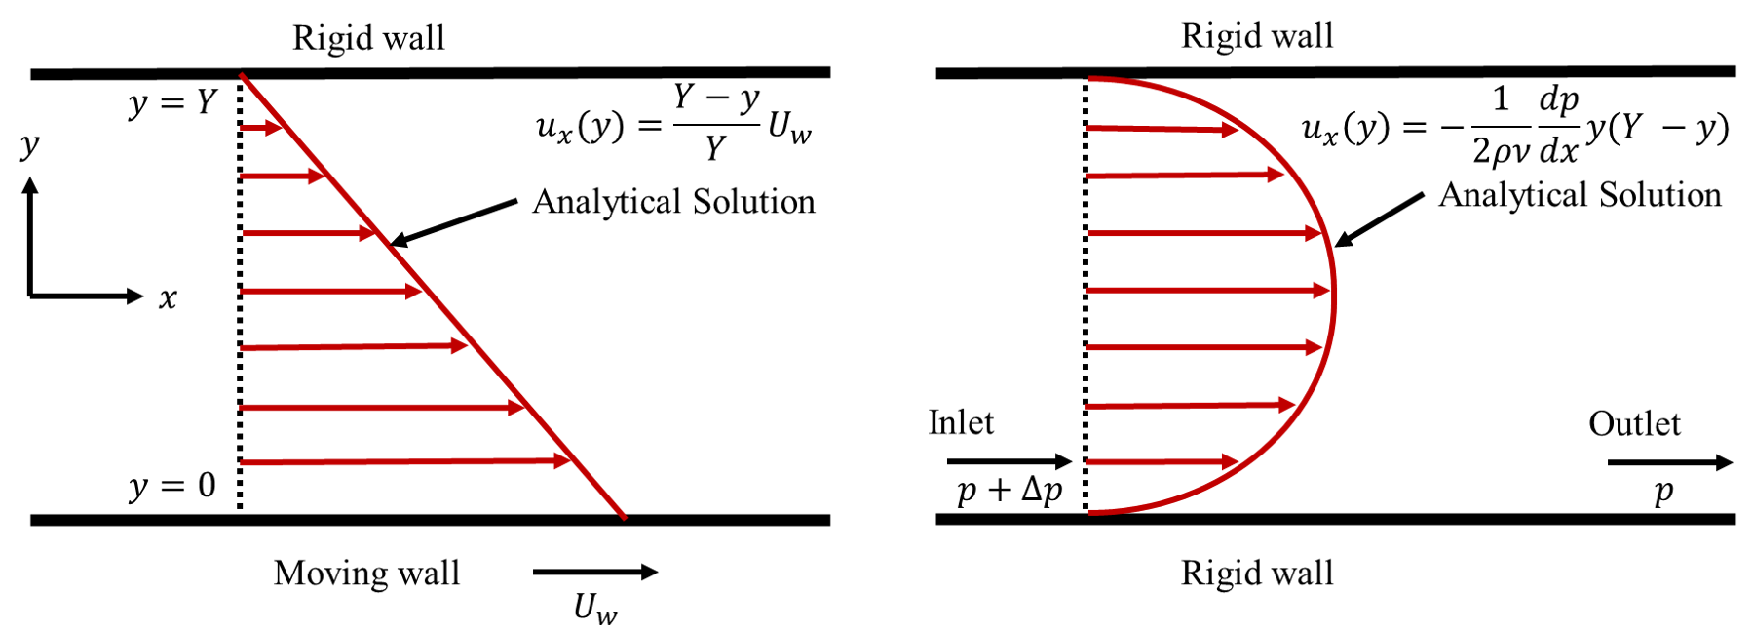
\includegraphics[width=0.98\textwidth]{imgs/couette_and_poiseuille.pdf}
  \caption{The conceptual visualizations of the Couette flow (Left) and
  Poiseuille flow (Right).}
  \label{couette-and-poiseuille-conceptual}
\end{figure}


\subsection{Couette flow}
The Couette flow is the flow between two walls as shown in Figure~\ref{couette-and-poiseuille-conceptual}:
One is fixed and the other moves horizontally at the velocity of $U_w$.
The flow is caused by the viscous drag force acting on the fluid.
Since the Couette flow also has an analytical solution,
we can validate the implementation of the moving wall.
The analytical solution for Figure~\ref{couette-and-poiseuille-conceptual} is given by:
\begin{equation}
\begin{aligned}
  u_x(y) =\frac{Y - y}{Y}U_w
\end{aligned}
\end{equation}
where $Y$ is the distance between the two walls
and $u_x(y)$ is the horizontal velocity of the flow
at the location of $y$. 
In the experiment, we apply the bounce-back boundary condition
at the moving wall and the rigid wall
and the periodic boundary conditions at the inlet and outlet.
The results are shown in Figure~\ref{fig:couette-velocity-evolution}.
As shown in the figures, the flow velocity iteratively approaches
the analytical solution and it perfectly fits in the end.
From this experiment, the moving wall can be validated.

\newpage
\begin{figure}[H]
  \begin{center}
    \subfloat[$t = 0$]{
      \includegraphics[width=0.44\textwidth]{../log/couette_flow/fig/couette_flow000000.pdf}
    }
    \subfloat[$t = 200$]{
      \includegraphics[width=0.44\textwidth]{../log/couette_flow/fig/couette_flow000200.pdf}
    }\\
    \subfloat[$t = 400$]{
      \includegraphics[width=0.44\textwidth]{../log/couette_flow/fig/couette_flow000400.pdf}
    }
    \subfloat[$t = 600$]{
      \includegraphics[width=0.44\textwidth]{../log/couette_flow/fig/couette_flow000600.pdf}
    }\\
    \subfloat[$t = 800$]{
      \includegraphics[width=0.44\textwidth]{../log/couette_flow/fig/couette_flow000800.pdf}
    }
    \subfloat[$t = 1000$]{
      \includegraphics[width=0.44\textwidth]{../log/couette_flow/fig/couette_flow001000.pdf}
    }\\
    \subfloat[$t = 1200$]{
      \includegraphics[width=0.44\textwidth]{../log/couette_flow/fig/couette_flow001200.pdf}
    }
    \subfloat[$t = 1400$]{
      \includegraphics[width=0.44\textwidth]{../log/couette_flow/fig/couette_flow001400.pdf}
    }
    \caption{The velocity evolution at
      the $x = 25$ in the lattice grid size of $(50, 50)$.
      The wall velocity $U_w$ and the relaxation term $\omega$ are set
      to $50$ and $0.3$ respectively.
      The initial density is $\rho(\xv) = 1.0$ and the initial velocity is $\uv(\xv) = (0, 0)$. 
      \label{fig:couette-velocity-evolution}}
  \end{center}
\end{figure}

\newpage
\subsection{Poiseuille flow}
The Poiseuille flow is the flow between two non-moving walls as shown in Figure~\ref{couette-and-poiseuille-conceptual}.
The flow is caused by a constant pressure difference $\od{p}{x}$
in the horizontal direction of the two walls.
The Poiseuille flow also has the analytical solution
and we can validate the implementation of the periodic boundary conditions
with pressure variation.
The analytical solution for Figure~\ref{couette-and-poiseuille-conceptual} is given by:
\begin{equation}
\begin{aligned}
  u_x(y) = - \frac{1}{2\rho \nu} \od{p}{x} y (Y - y)
\end{aligned}
\end{equation}
In the experiment, we apply the bounce-back boundary condition
at the moving wall and the rigid wall
and the periodic boundary condition with pressure variation at the inlet and outlet.
Figure~\ref{fig:poiseuille-velocity-evolution} presents the results
and the simulated results approaches the analytical solutions as in the Couette flow.
In the end, it fits completely.

\begin{figure}[H]
  \begin{center}
    \subfloat[$t = 0$]{
      \includegraphics[width=0.31\textwidth]{../log/poiseuille_flow/fig/poiseuille_flow000000.pdf}
    }
    \subfloat[$t = 500$]{
      \includegraphics[width=0.31\textwidth]{../log/poiseuille_flow/fig/poiseuille_flow000500.pdf}
    }
    \subfloat[$t = 1000$]{
      \includegraphics[width=0.31\textwidth]{../log/poiseuille_flow/fig/poiseuille_flow001000.pdf}
    }\\
    \subfloat[$t = 1500$]{
      \includegraphics[width=0.31\textwidth]{../log/poiseuille_flow/fig/poiseuille_flow001500.pdf}
    }
    \subfloat[$t = 2000$]{
      \includegraphics[width=0.31\textwidth]{../log/poiseuille_flow/fig/poiseuille_flow002000.pdf}
    }
    \subfloat[$t = 2500$]{
      \includegraphics[width=0.31\textwidth]{../log/poiseuille_flow/fig/poiseuille_flow002500.pdf}
    }\\
    \subfloat[$t = 3000$]{
      \includegraphics[width=0.31\textwidth]{../log/poiseuille_flow/fig/poiseuille_flow003000.pdf}
    }
    \subfloat[$t = 3500$]{
      \includegraphics[width=0.31\textwidth]{../log/poiseuille_flow/fig/poiseuille_flow003500.pdf}
    }
    \subfloat[$t = 4000$]{
      \includegraphics[width=0.31\textwidth]{../log/poiseuille_flow/fig/poiseuille_flow004000.pdf}
    }
    \caption{The velocity evolution at
      the $x = 25$ in the lattice grid size of $(50, 50)$.
      The relaxation term $\omega$ are is
      to $0.7$.
      The density factor at the inlet and the density factor
      at the outlet are set to $0.3$ and $0.301$ respectively.
      The initial density is $\rho(\xv) = 1.0$ and the initial velocity is $\uv(\xv) = (0, 0)$.
      \label{fig:poiseuille-velocity-evolution}}
  \end{center}
\end{figure}

\newpage
\section{Lid-driven cavity}
Finally, we handle a concrete example.
In this paper, the lid-driven cavity shown in Figure~\ref{lid-driven-cavity-conceptual} are simulated.
The lid-driven cavity simulates the flow inside a box with
three rigid walls and one moving wall, i.e. a lid.
In this simulation, it is known that the turbulence is caused 
when the following Reynolds number is larger than 1000:
\begin{equation}
\begin{aligned}
  \text{Re} = \frac{LU}{\nu}
\end{aligned}
\end{equation}
where $L$ is the characteristic length parameter
of the body and $U$ is the stream flow velocity.
One key property of the Reynolds number is that two flow system
is dynamically similar if the Reynolds number and the geometry are similar.
Therefore, we present the results with various 
viscosity $\nu$ and the wall velocity $U = U_w$ that 
satisfy the Reynolds number of $1000$ under $L = X = Y = 300$
in Figure~\ref{fig:sliding-lid-velocity-evolution}.
As the viscosity and velocity becomes larger,
the convergence becomes quicker.
On the other hand, all the settings converge to the similar flow in the end
as indicated in the key property of the Reynolds number.

\begin{figure}
  \centering
  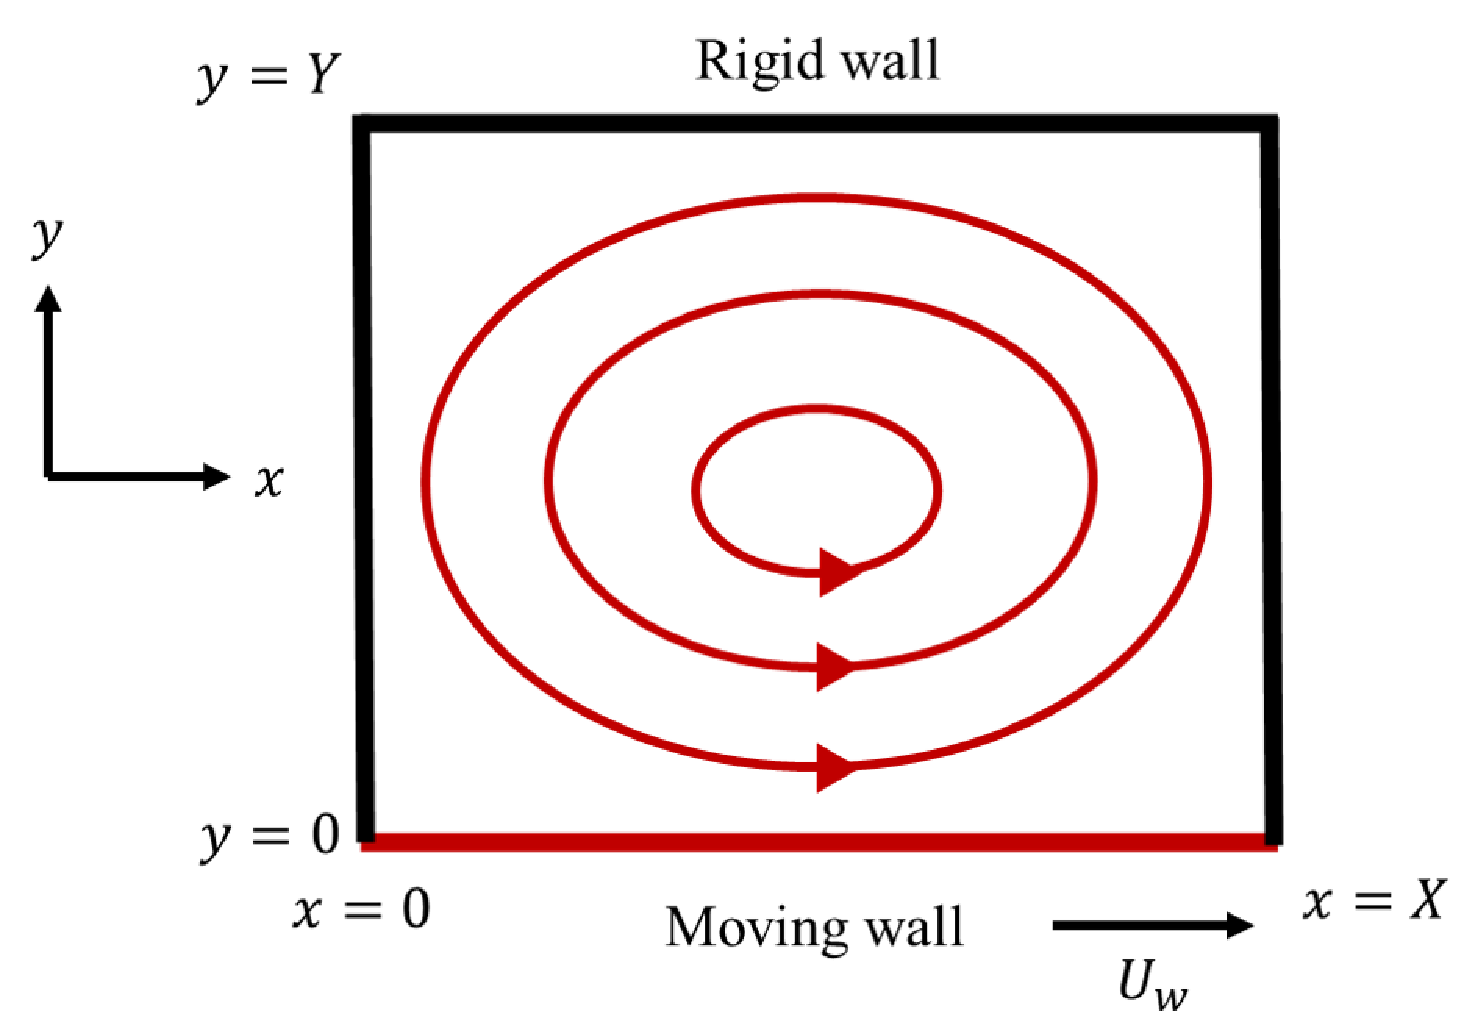
\includegraphics[width=0.68\textwidth]{imgs/lid-driven-cavity.pdf}
  \caption{The conceptual visualizations of the lid-driven cavity.}
  \label{lid-driven-cavity-conceptual}
\end{figure}

\begin{figure}[H]
  \begin{center}
    \subfloat[$t = 5000$]{
      \includegraphics[width=0.23\textwidth]{../log/sliding_lid_W0.10_visc0.03_size300/fig/vel_flow005000.pdf}
    }
    \subfloat[$t = 10000$]{
      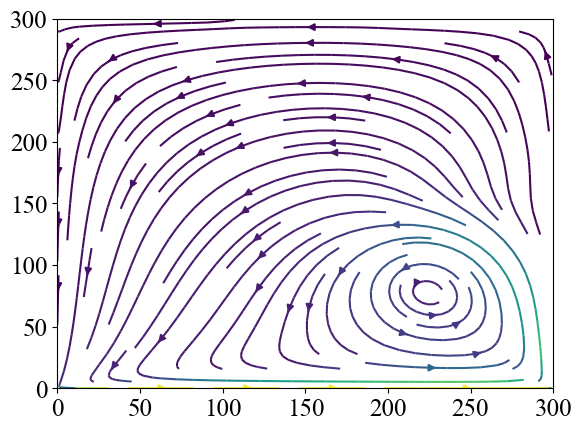
\includegraphics[width=0.23\textwidth]{../log/sliding_lid_W0.10_visc0.03_size300/fig/vel_flow010000.pdf}
    }
    \subfloat[$t = 50000$]{
      \includegraphics[width=0.23\textwidth]{../log/sliding_lid_W0.10_visc0.03_size300/fig/vel_flow050000.pdf}
    }
    \subfloat[$t = 100000$]{
      \includegraphics[width=0.23\textwidth]{../log/sliding_lid_W0.10_visc0.03_size300/fig/vel_flow095000.pdf}
    }\\
    \subfloat[$t = 5000$]{
      \includegraphics[width=0.23\textwidth]{../log/sliding_lid_W0.20_visc0.06_size300/fig/vel_flow005000.pdf}
    }
    \subfloat[$t = 10000$]{
      \includegraphics[width=0.23\textwidth]{../log/sliding_lid_W0.20_visc0.06_size300/fig/vel_flow010000.pdf}
    }
    \subfloat[$t = 50000$]{
      \includegraphics[width=0.23\textwidth]{../log/sliding_lid_W0.20_visc0.06_size300/fig/vel_flow050000.pdf}
    }
    \subfloat[$t = 100000$]{
      \includegraphics[width=0.23\textwidth]{../log/sliding_lid_W0.20_visc0.06_size300/fig/vel_flow095000.pdf}
    }\\
    \subfloat[$t = 5000$]{
      \includegraphics[width=0.23\textwidth]{../log/sliding_lid_W0.30_visc0.09_size300/fig/vel_flow005000.pdf}
    }
    \subfloat[$t = 10000$]{
      \includegraphics[width=0.23\textwidth]{../log/sliding_lid_W0.30_visc0.09_size300/fig/vel_flow010000.pdf}
    }
    \subfloat[$t = 50000$]{
      \includegraphics[width=0.23\textwidth]{../log/sliding_lid_W0.30_visc0.09_size300/fig/vel_flow050000.pdf}
    }
    \subfloat[$t = 100000$]{
      \includegraphics[width=0.23\textwidth]{../log/sliding_lid_W0.30_visc0.09_size300/fig/vel_flow095000.pdf}
    }\\
    \subfloat[$t = 5000$]{
      \includegraphics[width=0.23\textwidth]{../log/sliding_lid_W0.40_visc0.12_size300/fig/vel_flow005000.pdf}
    }
    \subfloat[$t = 10000$]{
      \includegraphics[width=0.23\textwidth]{../log/sliding_lid_W0.40_visc0.12_size300/fig/vel_flow010000.pdf}
    }
    \subfloat[$t = 50000$]{
      \includegraphics[width=0.23\textwidth]{../log/sliding_lid_W0.40_visc0.12_size300/fig/vel_flow050000.pdf}
    }
    \subfloat[$t = 100000$]{
      \includegraphics[width=0.23\textwidth]{../log/sliding_lid_W0.40_visc0.12_size300/fig/vel_flow095000.pdf}
    }\\
    \caption{The stream plots of sliding lid
    with the lattice grid size of $(300, 300)$.
    Figure~(a) -- (d) are the results of 
    the viscosity $\nu = 0.03$ and the wall velocity $0.1$.
    Figure~(e) -- (h) are the results of 
    the viscosity $\nu = 0.06$ and the wall velocity $0.2$.
    Figure~(i) -- (l) are the results of 
    the viscosity $\nu = 0.09$ and the wall velocity $0.3$.
    Figure~(m) -- (p) are the results of 
    the viscosity $\nu = 0.12$ and the wall velocity $0.4$.
    Note that each setting is chosen to satisfy
    the Reynolds number 1000.
    The initial density is $\rho(\xv) = 1.0$ and the initial velocity is $\uv(\xv) = (0, 0)$.
      \label{fig:sliding-lid-velocity-evolution}}
  \end{center}
\end{figure}

This experiment requires long time to complete the experiments.
For example, it takes 1 hour to finish one simulation using
intel core i7--10700 and 32GB RAM.
Recall that the advantage of LBM is that it allows us to compute the simulation in
parallel easily.
For this reason, we test the scalability of this simulation using
various number of processors.
Figure~\ref{fig:sliding-lid-scaling} shows the plot of
MLUPS, a.k.a. million lattice updates per second, and
the number of processors.
Ideally, the MLUPS grows linearly with respect to the number of processors.
However, it does not happen because of the latency of the communication
and the waiting for the synchronization.
Such slow down is also seen in the results.
\begin{figure}
  \centering
  \includegraphics[width=0.58\textwidth]{../log/sliding_lid_W0.10_visc0.03_size300/fig/scaling_test.pdf}
  \caption{The scaling test of the sliding lid simulation.
  The grid size is $300 \times 300$.
  The number of processes are $1 ,4 ,9 ,16 ,25 ,36 ,100 ,144 ,225 ,400$ respectively.
  Note that both axes are log-scale.
    The viscosity and the wall velocity are set to $\nu = 0.03$ and $0.1$.
    The initial density is $\rho(\xv) = 1.0$ and the initial velocity is $\uv(\xv) = (0, 0)$.
  }
  \label{fig:sliding-lid-scaling}
\end{figure}

